\documentclass[a4paper]{article}

\usepackage[T1]{fontenc}
\usepackage[utf8]{inputenc}
\usepackage{lmodern}

\usepackage{graphicx}
\usepackage[english]{babel}
\usepackage{csquotes}

\usepackage{subcaption}
\usepackage{booktabs}

\usepackage{biblatex}
\addbibresource{bibliography.bib}


\linespread{1.25}

\title{HiSVis: Scene Detection in Historical Photo Collections}
\author{Melvin Wevers}
\date{\today}
 
\begin{document}
 
\maketitle
 
\section{Introduction}
Computer Vision algorithms have become capable identifying objects and scenes in images with high accuracy. While computer vision algorithms are commonplace in self-driving cars, drone technology, or the analysis of social media posts, their use for heritage institutes has only recently been growing\autocite{bhargav_deep_2019}


%\cite{bhargav_deep_2019,bell_computing_2018,mager_visual_2020, niebling_analyzing_2020} 

The benefits for heritage institutes range from automatically enriching collections, to improving search capabilities, or enabling large-scale analysis of visual collections. 

%While computer vision technology advanced drastically in the last few years, many of the state-of-the-art models have been trained on contemporary data. This impacts the model's accuracy and applicability to heritage collections. The ability to detect objects from the past that looked noticeably different is difficult for such models. Not only have objects changed, the medium itself has also changed, granting contemporary data with a different visual style.  Compare, for example, a grainy black and white image of a traffic situation in the 1950s to a high-resolution color image taken with a zoom lens of a highway in 2020. Not only do the cars look different, but the use of color and the abilities of cameras yield pictures that look very different. 
%
%One approach to counter this lack of models trained on historical data is to feed historical material to existing models and fine tune their performance. This builds upon the categories existent in the modern datasets. However, these categories do not always map onto the categories present in the collections of heritage institutes, or they do not align with the search interests of users. A different approach is transfer learning, which builds upon existing models by adding new categorizations, which are trained using the historical material. Because the models have already been pretrained with large collections of images, often only a small number of images is needed to learn a new category. Of course, this depends on the complexity of the category and the diversity present in the training data. 
%
%This paper presents a use case of how transfer learning can be employed to images from a historical photo collection. We focus on one particular computer vision task: scene detection. This task does not describe the existence of a particular object in a picture, or draws bounding boxes around these objects, but rather tries to describe ``the place in which the objects seat.''\cite{zhou_places_2018} Oliva and Torrabla write that humans can quickly recognize the functional and categorical properties of a scene, while overlooking the objects and locations in a scene \cite{oliva_modeling_2001}. The ability to search for images based on the scene represented in them is a useful feature, especially since this information is often not included in the meta data. 
%
%More specifically, we explore how transfer learning can be applied to \textit{Places365}, a scene detection model. We will reflect on the creation of the training data, the training strategy, as well as the evaluation of the model. Finally, we discuss the added benefits of this type of computer vision algorithm for heritage institutes and archives. 
%
%
%\section{Data}
%
%This dataset for this study is the photo collection of press agency \textit{De Boer} for the period 1945-2004.\footnote{This data has been provided by the \textit{Noord-Hollands Archief}.} The \textit{De Boer} collection focuses on national and regional events, although over time the collection's focus gradually shifted to the region Kennemerland. This region, just north of Amsterdam, includes cities such as Haarlem, Zandvoort, Bloemendaal, and Alkmaar.
%%
%The value of the collection was recognized locally, nationally, and internationally. In 1962, the founder of this prestigious photo collection, Cees de Boer, was awarded the World Press Photo and the Silver Camera (\textit{Zilveren Camera}). Cees' son Joppe won the national photo journalist award in 1969. The press agency provided pictures to the Regional newspaper \textit{Haarlems Dagblad}. The photo collection depicted a wide range of events, ranging from the first and only show of The Beatles in Blokker, the arrival of Martin Luther King in 1964, to opening of restaurants, and sport events (see Figure~\ref{fig:example}).
%
%\begin{figure}
%	\centering
%  	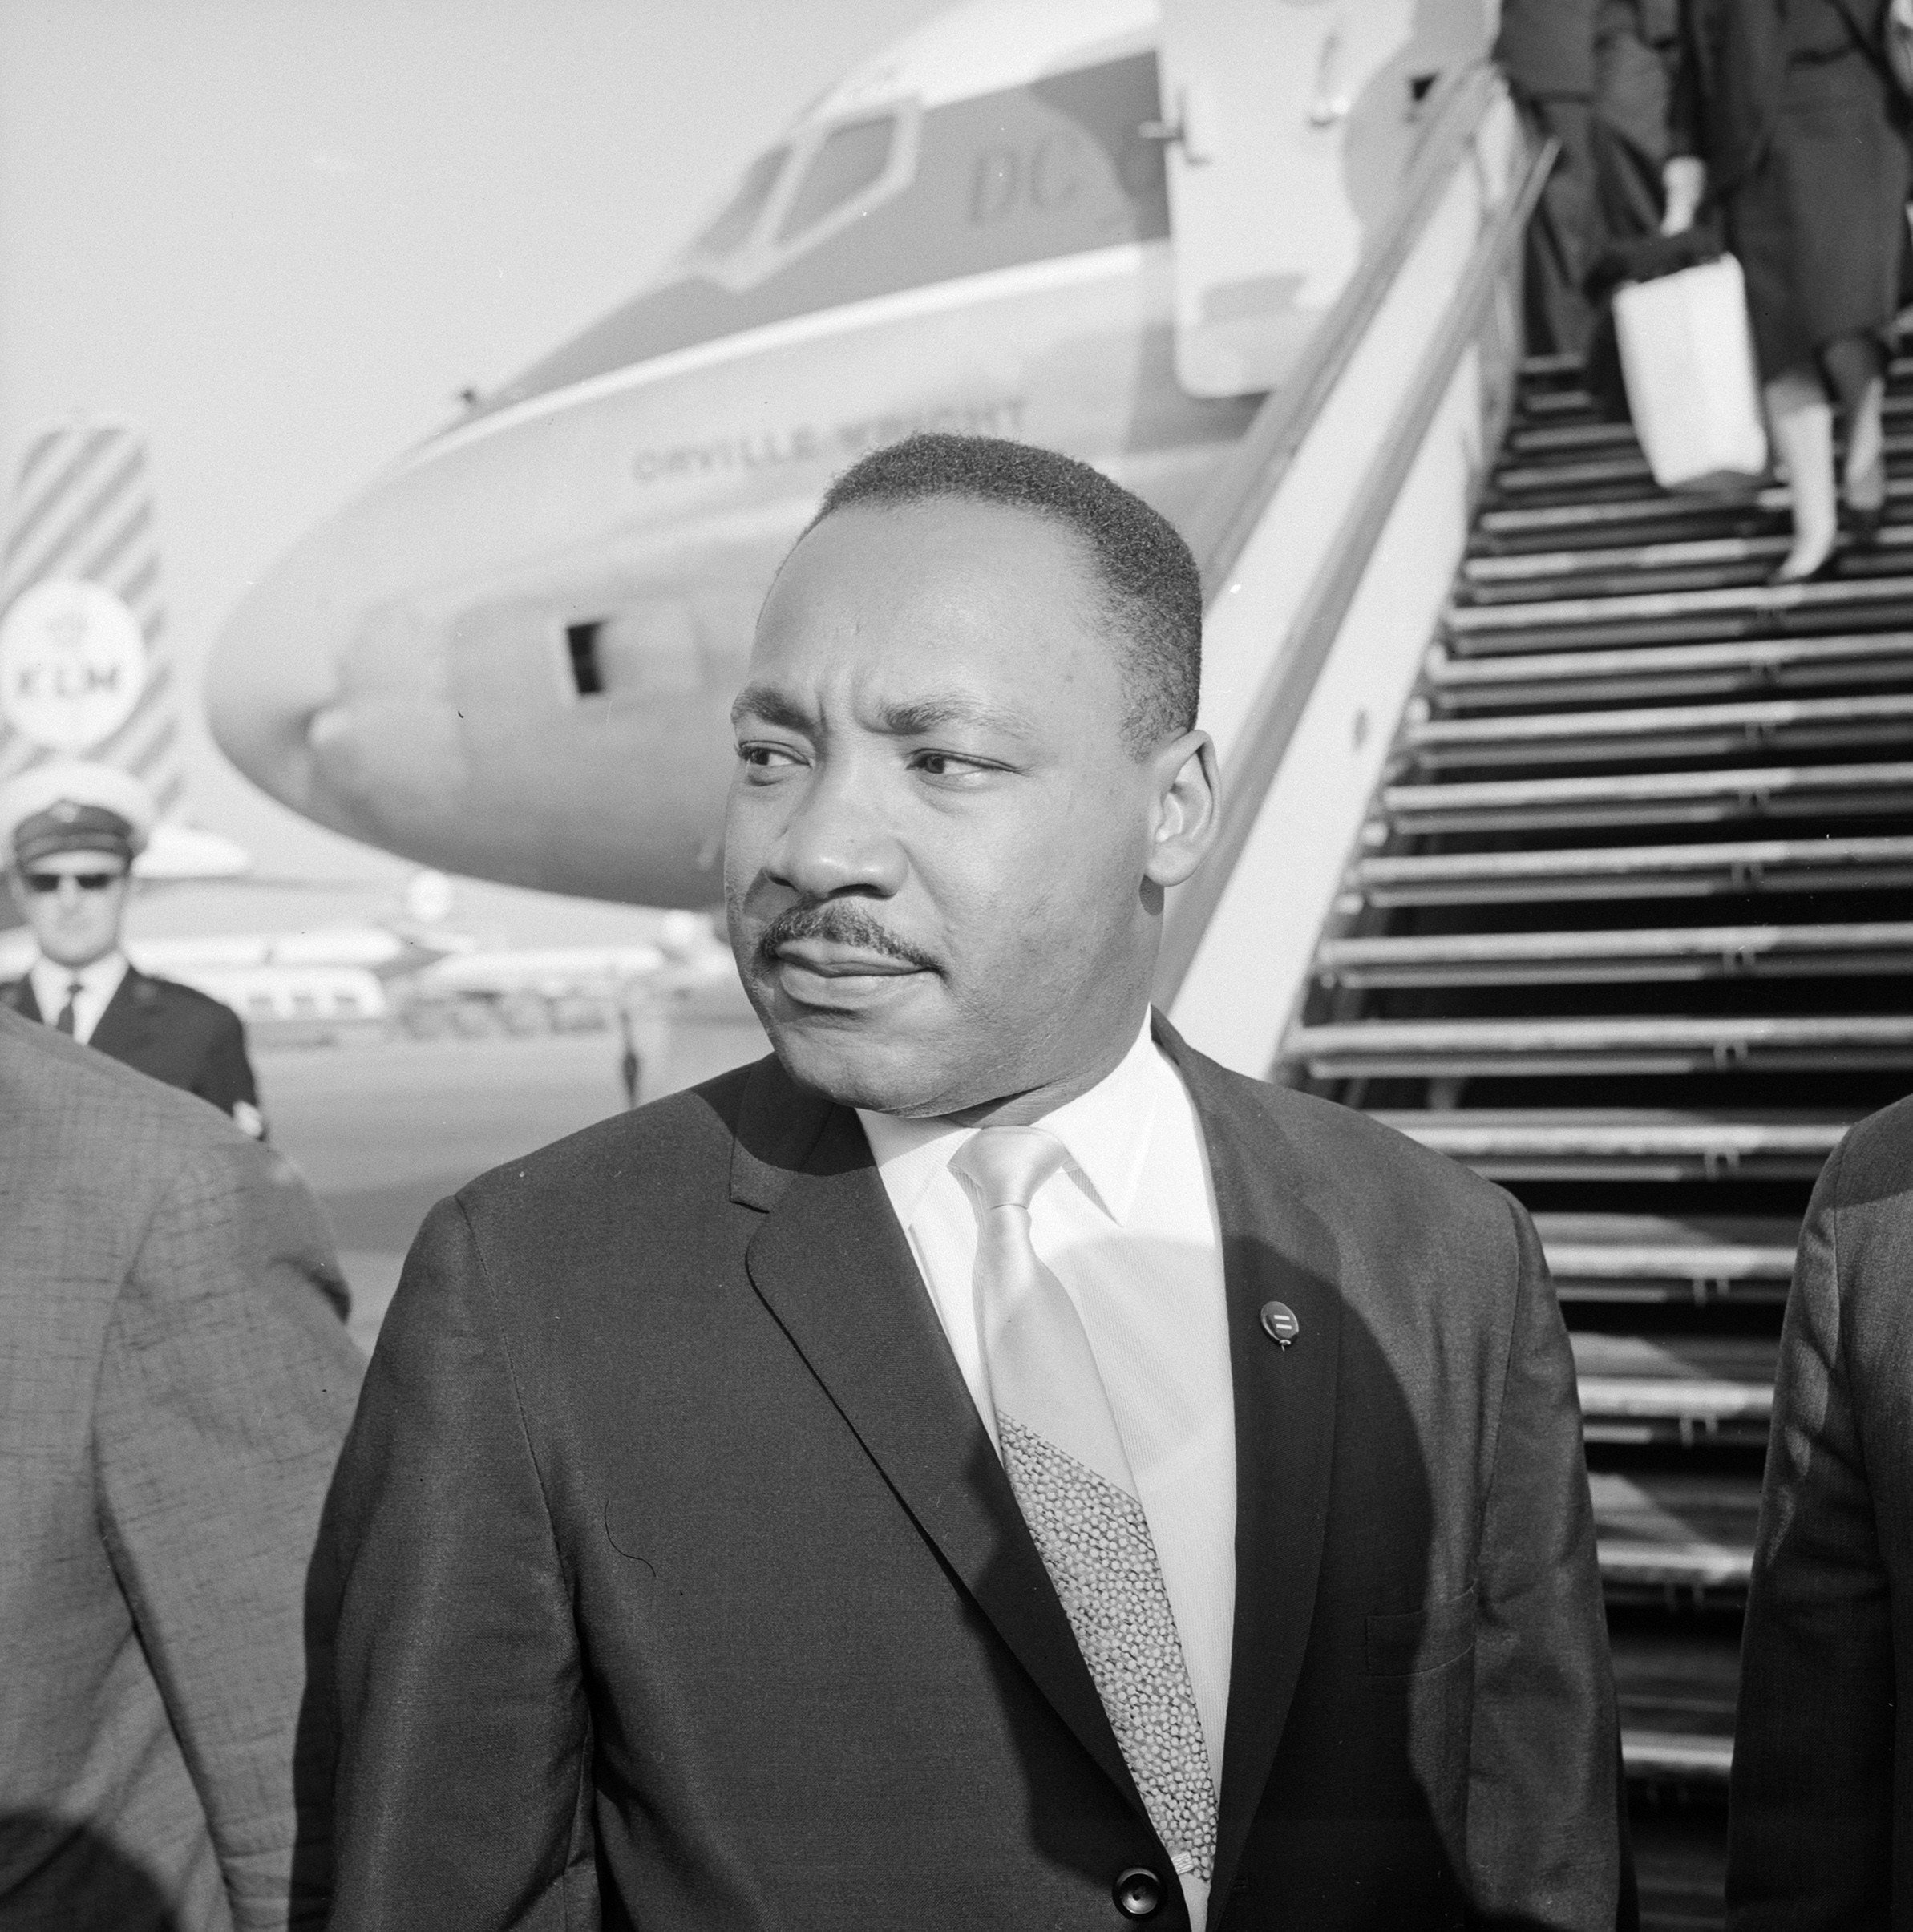
\includegraphics[width=0.5\textwidth]{../output/figures/NL-HlmNHA_1478_1926 A_07.jpg}
%  	\caption{Arrival of Martin Luther King Jr. at Schiphol Airport, August 15, 1964.}
%  	\label{fig:example}
%\end{figure}
%
%The photo collection consists of approximately two million negatives and metadata for the period 1945-2004. The metadata is based on topic cards and logs kept by the photo agency. On these topic cards, the agency detailed what was depicted on the pictures. For the period 1952-1990, these logs have been transcribed using volunteers. The negatives of the pictures are currently being digitized, and these digitized photographs will be linked to the metadata. As part of this digitization process, subsets of photographs will be annotated using the topic cards and manual annotators. These annotations will be used to train computer vision algorithms to further augment the dataset and to create models trained on historical photo collection. 
%
%This study explores the usefulness of scene detection for this particular collection. For this, we relied on a subset of data that had already been digitized by the \textit{Noord-Hollands Archief}. This subset consisted of 2,545 images from their online repository, an early batch of digitized images, and digitized small negatives. 
%
%We took the categorization scheme for Places-365 as a starting point. As the name implies, this scheme contains 365 categories of scenes, ranging from `alcove' to `raft'.\footnote{An overview of the categories can be found here: \url{http://places2.csail.mit.edu/explore.html}}. We combined this scheme with information from the catalogue cards that the Boer used. These catalogue cards could not be linked to the categorization scheme directly, because these cards often contain categories that are too specific or category that were not visually represented. Making categories is always a trade-off between specificity and reductionism. In making these categories, we kept in mind whether there remained an historical and visual consistency within the categories \textit{and} if the category would be of use for users of the collection. 
%
%%% TODO: add part about survey
%
%Together with archivists and cultural historians, we studied the images in the training set and devised a categorization scheme of 159 categories.\footnote{In the appendix, we added annotation guidelines, which will be used for the annotation of the further dataset.} During annotation, we noticed the difficulties in separating scenes that were characterized by a particular object from scenes defined by the location or the action performed in the image. The developers of the SUN database, another scene image set, describe how scenes are linked to particular functions and behaviors, which are closely tied to the visual features that structure the space. Large rooms or areas allow for different types of behavior.\cite{xiao2010sun} This description alludes to the complexity of the notion of a scene.\cite{xie_scene_2020} Moreover, there is a large inter-class similarity between scenes, for example, between library and bookstore, while concurrently, we see intra-class variations, in which images within a category are very diverse.
%
%The distribution of these images is heavily skewed as can be seen in Figure~\ref{fig:categories}. The categories `soccer' and 'construction site' are very well represented, while most others appeared much more infrequently. For training, we removed categories with less than 20 images, this included categories such as: `house\_boat', `castle', and `campsite'. When annotating the larger dataset for training purposes, we intend to again include these categories. Moreover, during annotation, we will iteratively evaluate the training categories and possibly add new categories, or merge existing ones. 
%
%
%\begin{figure}
%  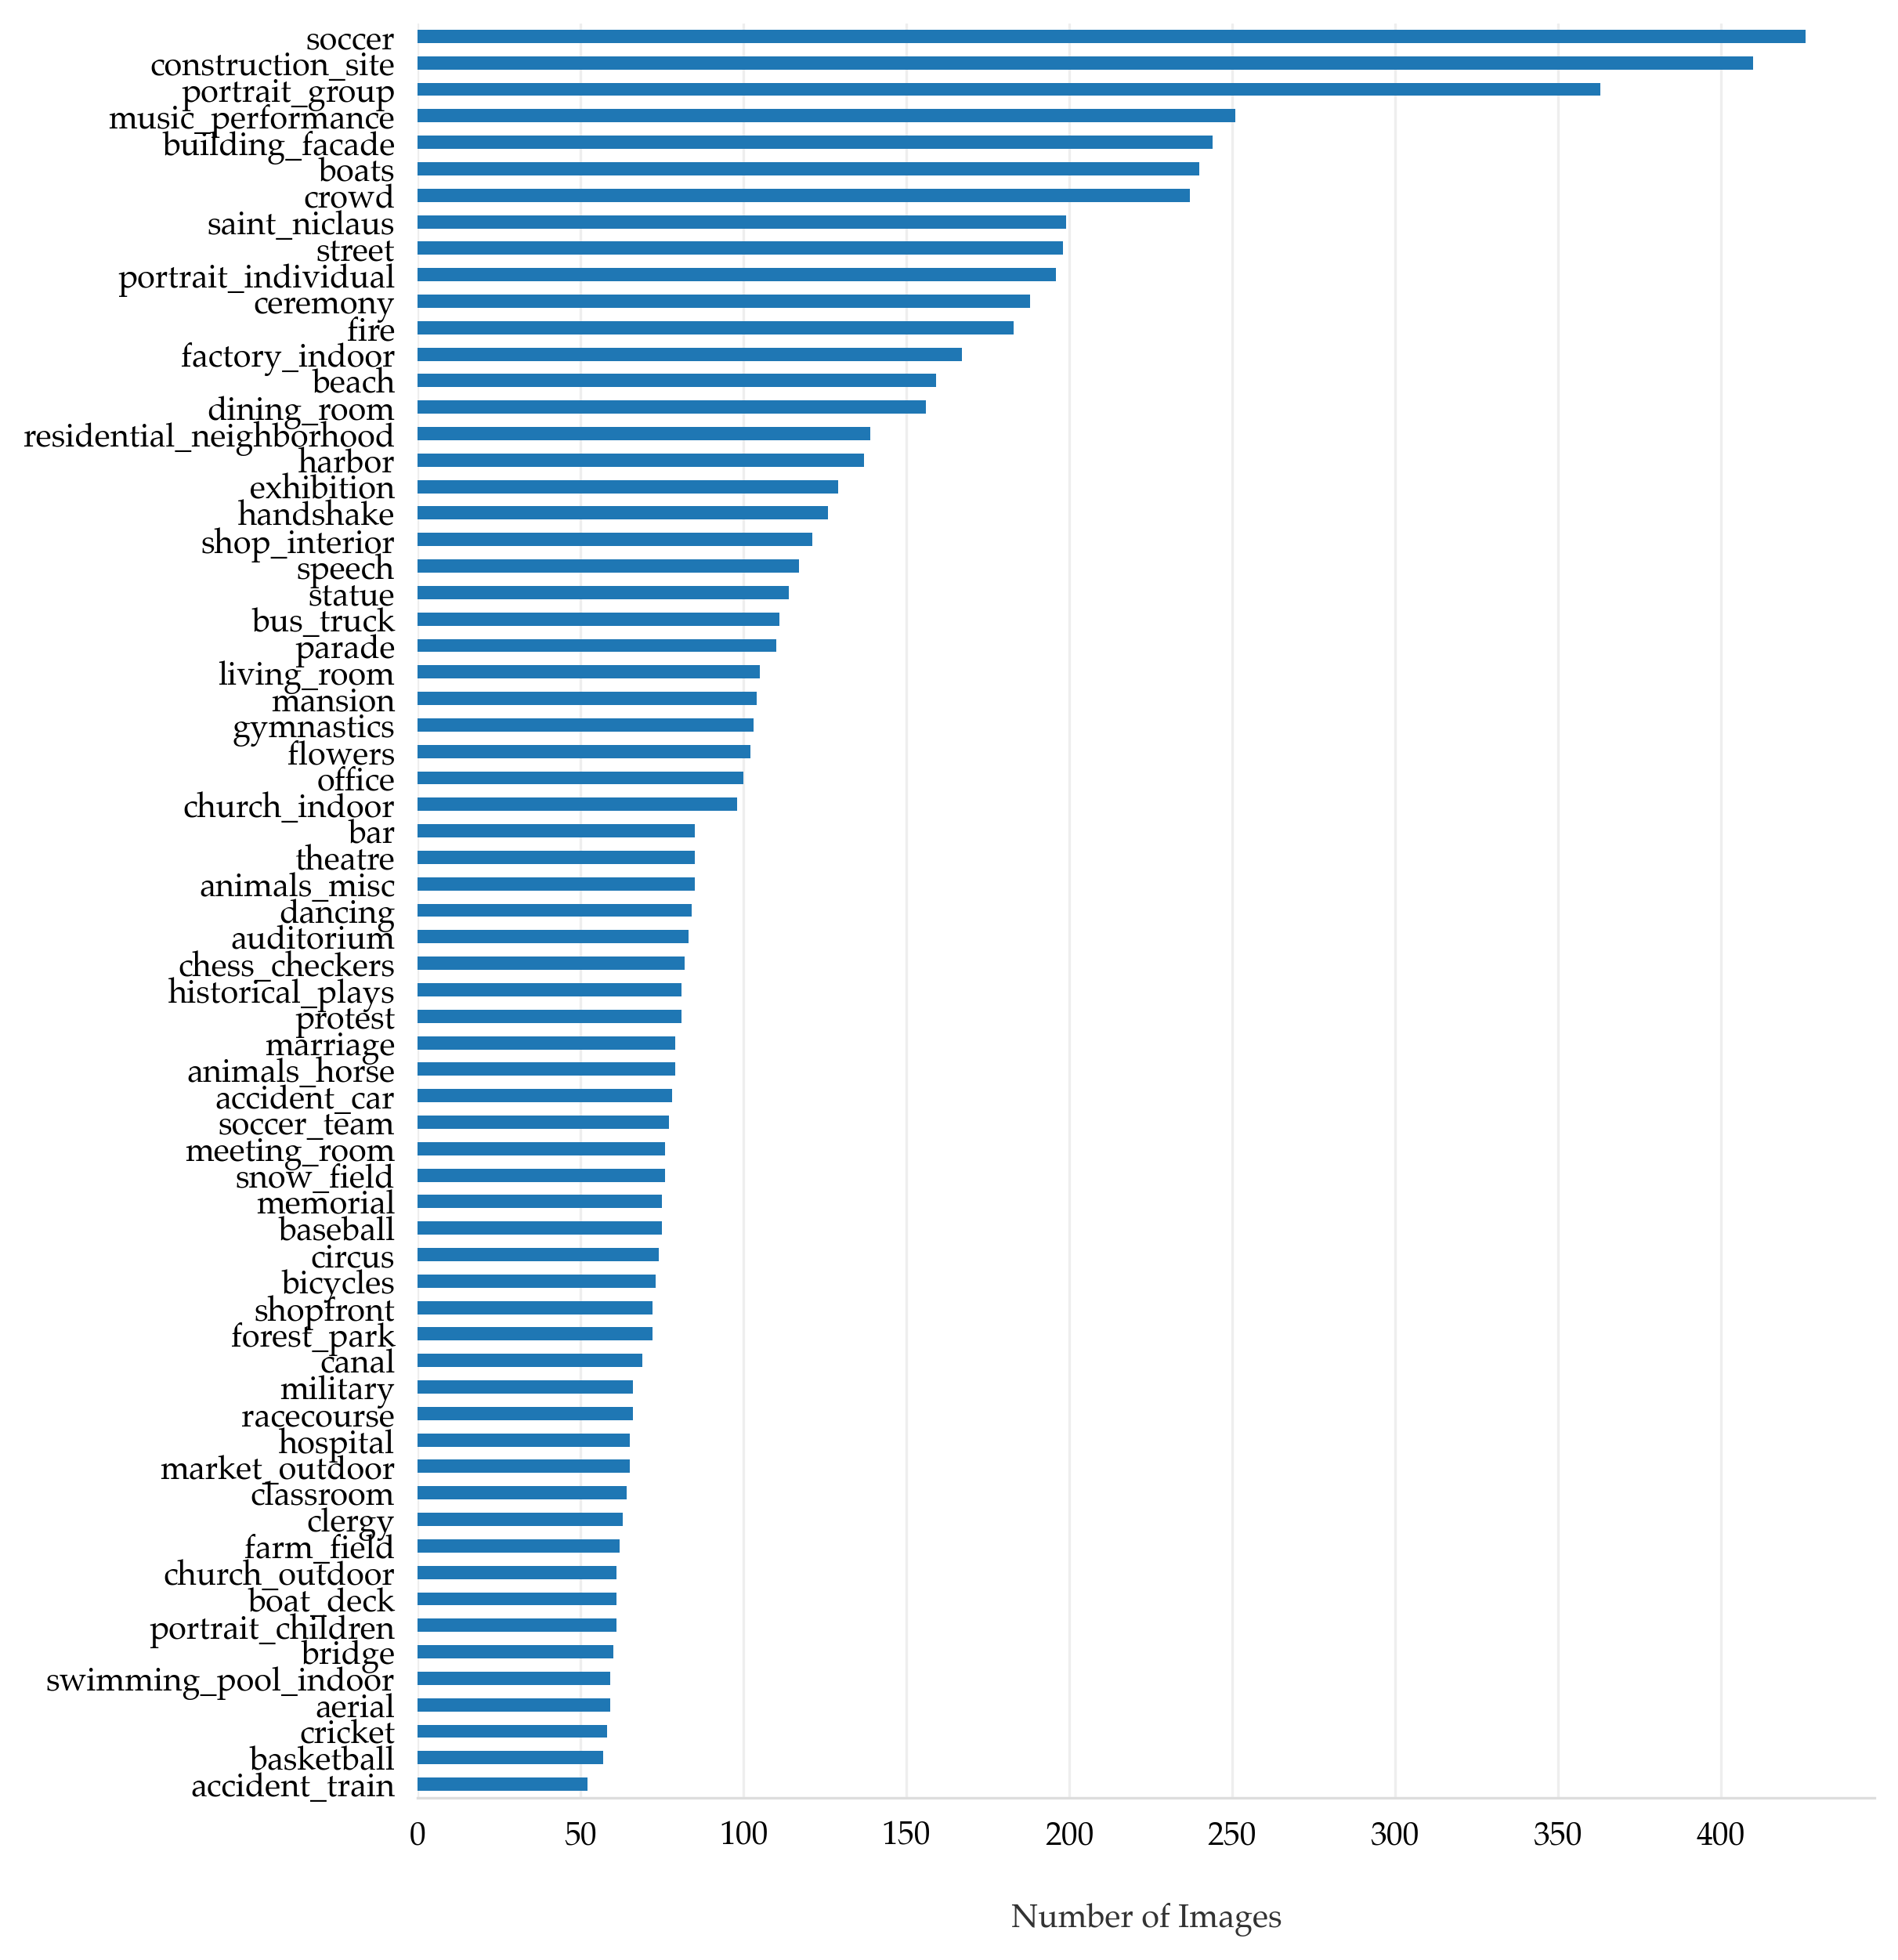
\includegraphics[width=0.95\textwidth]{../output/figures/categories.png}
%  \caption{Distribution of categories in training set.}
%  \label{fig:categories}
%\end{figure}
%
%\section{Method: Scene Detection}
%In the context of a heritage institute, scene detection is a useful task. Pictures in this historical photo collection are diverse and more often than not contain more than just an object or groups of objects. The photographs depicts events or scenes, such as memorials, construction sites, or parade (see Figure~\ref{fig:examples}). Even though example images are characterized by particular objects, they cannot be described just by the object. At the same time, the collection also included images that can accurately be described by an object (see Figure~\ref{fig:examples_objects}).
%
%\begin{figure}
%
%  \begin{subfigure}[b]{0.3\textwidth}
%    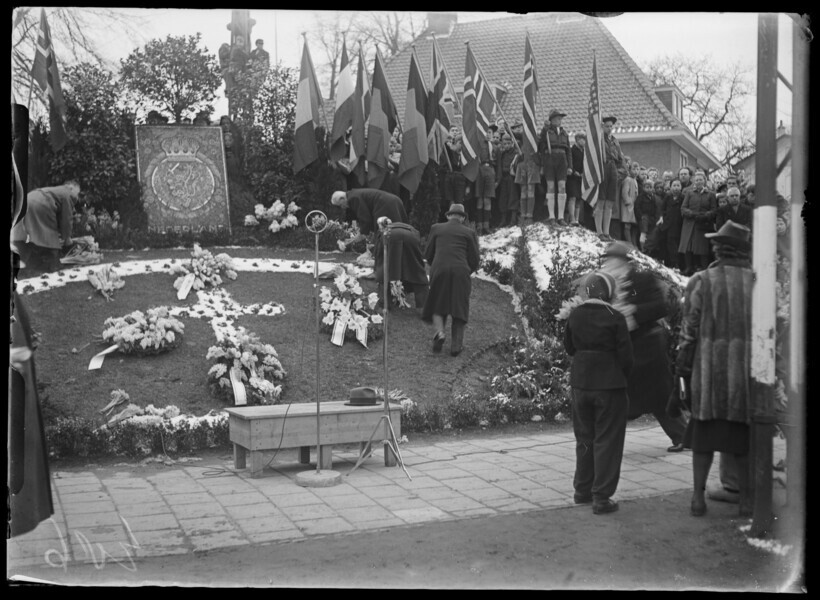
\includegraphics[width=\textwidth]{../output/figures/memorial.jpg}
%    \caption{Memorial}
%    \label{fig:examplesa}
%  \end{subfigure}
%  %
%  \begin{subfigure}[b]{0.3\textwidth}
%    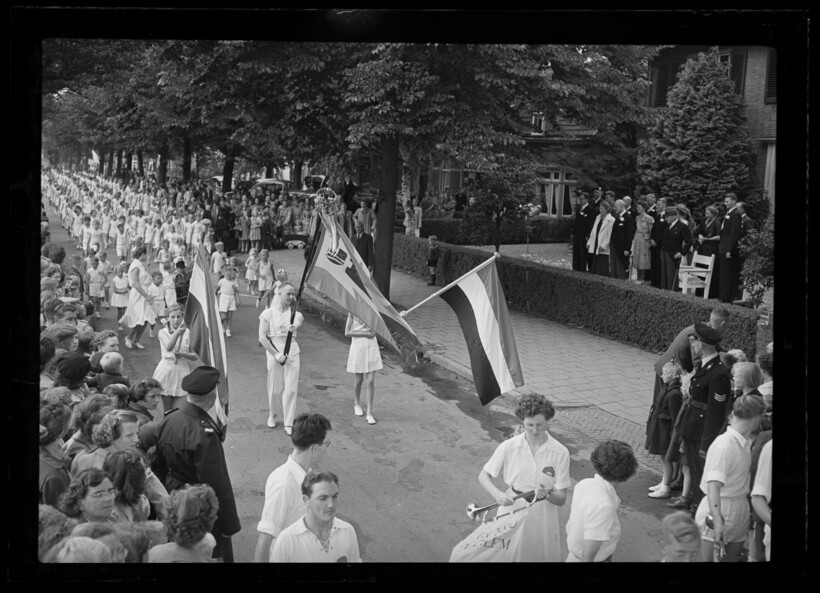
\includegraphics[width=\textwidth]{../output/figures/parade.jpg}
%    \caption{Parade}
%    \label{fig:examplesb}
%  \end{subfigure}
%  %
%  \begin{subfigure}[b]{0.3\textwidth}
%    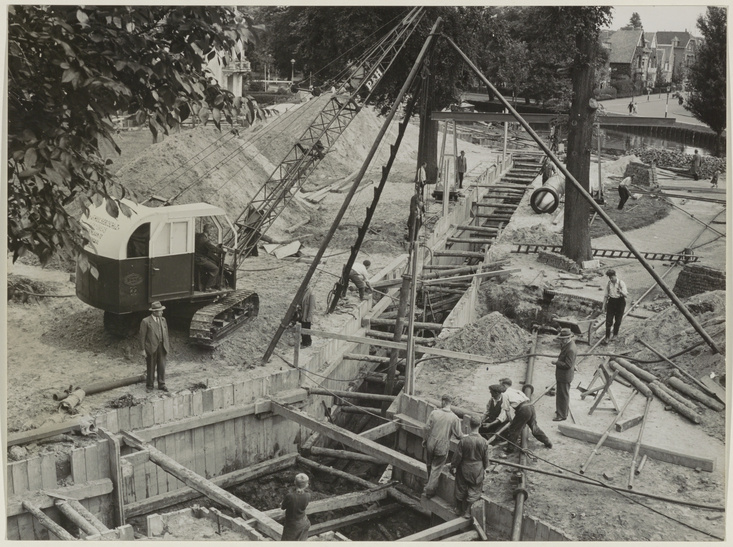
\includegraphics[width=\textwidth]{../output/figures/construction_site.jpg}
%    \caption{Construction Site}
%    \label{fig:examplesc}
%  \end{subfigure}
%   \caption{Three examples of scenes from \textit{De Boer} collection.}
%   \label{fig:examples}
%\end{figure}
%
%
%\begin{figure}
%
%  \begin{subfigure}[b]{0.3\textwidth}
%    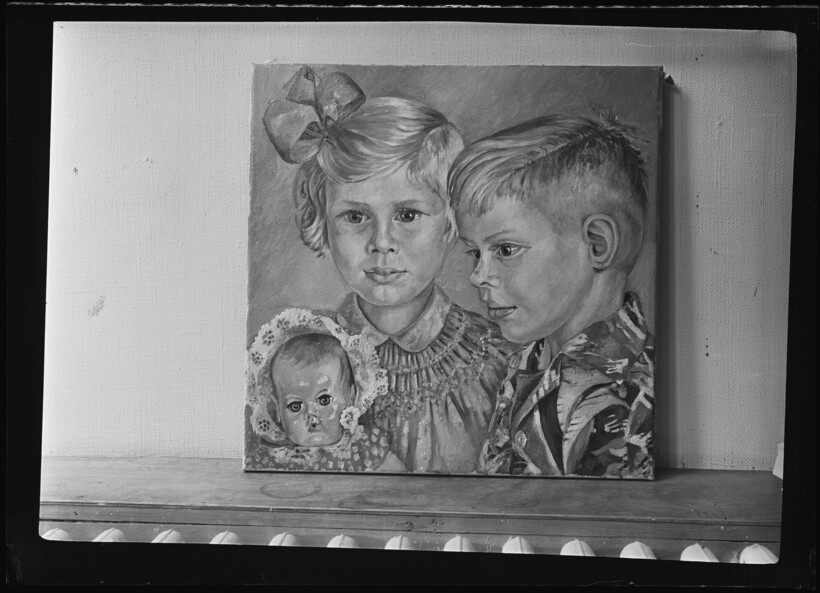
\includegraphics[width=\textwidth]{../output/figures/artwork.jpg}
%    \caption{Memorial}
%    \label{fig:examplesa}
%  \end{subfigure}
%  %
%  \begin{subfigure}[b]{0.3\textwidth}
%    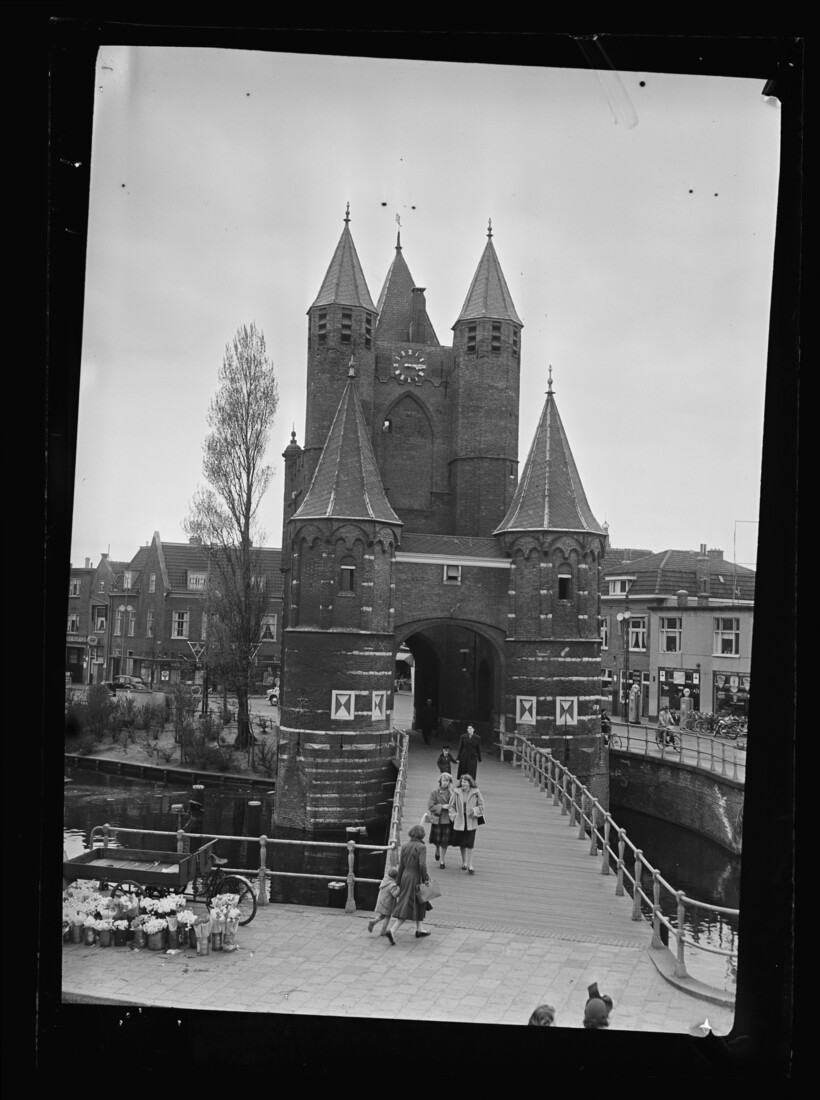
\includegraphics[width=\textwidth]{../output/figures/castle.jpg}
%    \caption{Parade}
%    \label{fig:examplesb}
%  \end{subfigure}
%  %
%  \begin{subfigure}[b]{0.3\textwidth}
%    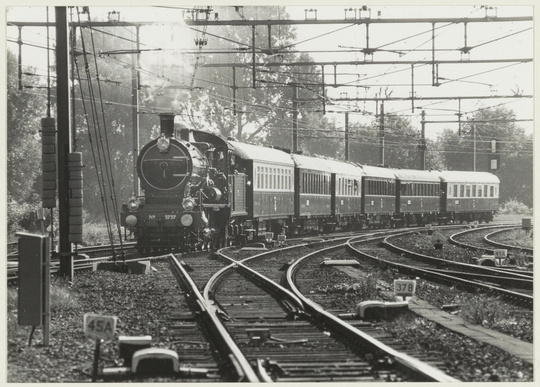
\includegraphics[width=\textwidth]{../output/figures/train.jpg}
%    \caption{Construction Site}
%    \label{fig:examplesc}
%  \end{subfigure}
%   \caption{Three examples of scenes characterized by a central object from \textit{De Boer} collection.}
%   \label{fig:examples_objects}
%\end{figure}
%
%We also explored object detection algorithms, but these required more extensive annotation to be able to detect particular objects in historical images. Moreover, merely detecting objects in images did not immediately yield useful categories. For example, for a picture of shopping street, object detection would identify people, bags, and perhaps a traffic light. In addition to extending the available categories to the historical collection, we also need to construct a conceptual framework for connecting these objects to overarching categories. In future work, we would like to further explore this line of research. For this study, we propose a computational approach that recognizes scene categories without any segmentation and the detection of individual objects. 
%
%As a starting point, we use a model trained on the Places-365 dataset. The authors of this dataset describe a scene as an ``environment(s) in the world, bounded by spaces where a human body would fit.''\cite{zhou_places_2018} The places models outperform ImageNet-CNN on scene-related datasets, underscoring the benefit of using such models for scene-related task over other models, such as ImageNet. The places365 dataset builds upon the SUN database, consisting of 899 categories with short descriptions.\footnote{https://groups.csail.mit.edu/vision/SUN/} For our annotation guidelines, we used the SUN descriptions as a starting point. Given that our dataset consists primarily out of black and white images, it is worth noting that these images were excluded from the SUN data. 
%
%For the scene detection in this dataset, we turn to transfer learning. This method refers to using ``what has been learned in one setting [...] to improve generalization in another setting.''\cite{goodfellow_deep_2016} In our case, we use what has been learned about scenes in the Places365-models to learn how to detect the scenes in our collection according to our categorization scheme. 
%
%The model we use as a point of departure for transfer learning is the ResNet50-places365 model, which as been trained on the Places365-Standard dataset, consisting of ~1.8 million images from 365 scene categories. This model reaches a 54.74\% top-1 accuracy and 85.08\% top-5 accuracy on the validation set. Top-1 accuracy is the percentage of images where the predicted label with the highest probablity matches the ground-truth label. Top-5 accuracy calculates whether the ground-truth label is in the top-five predicted labels. Because of the ambiguity between scene categories, top-5 accuracy is seen as a more suitable criterion.\cite{zhou_places_2018}
%
%
%For the training, we create a random validation set, containing 20 percent of the training images. We load a pretrained-Places365 model, for which we unfreeze the final fully-connected layers, add a ReLU layer, a dropout layer, a LogSoftmax layer, and the AdamW optimizer.\footnote{We also experimented with different drop out values, and unfreezing of deeper layers}. In simple terms, this means that we remove the part in which the classifications are made, and use the learned information stored in deeper layers to make new classifications using the new material as training data. To account for the small number of training data and to prevent overfitting, we apply data augmentations, dropout, and early stopping. 
%
%Next, we train the model for a maximum of 100 epochs, with an early stopping set at 5 epochs. To counter for the imbalance of the training categories, we experimented with weight-balancing the training data. 
%
%
%\section{Results}
%The mean top1-accuracy for tenfold cross-validation is 50.29 with a considerable standard deviation of 24.25. The top5-accuracy is 79.70 with a standard deviation of 18.69. 
%
%There were four categories (motorcycle, beauty salon, funeral, accident stretcher) with a top1-accuracy of 0, meaning that were never correctly identified. Closer inspections showed that the category `accident stretcher' might actually be the problem. This category actually refers to an object, while the predicted labels referred to where the stretcher was placed, soccer field or construction site, or more generally predicted the scene as a hospital. Appendix B contains a table with the accuracies for all the categories.
%
%\begin{figure}
%	\centering
%  	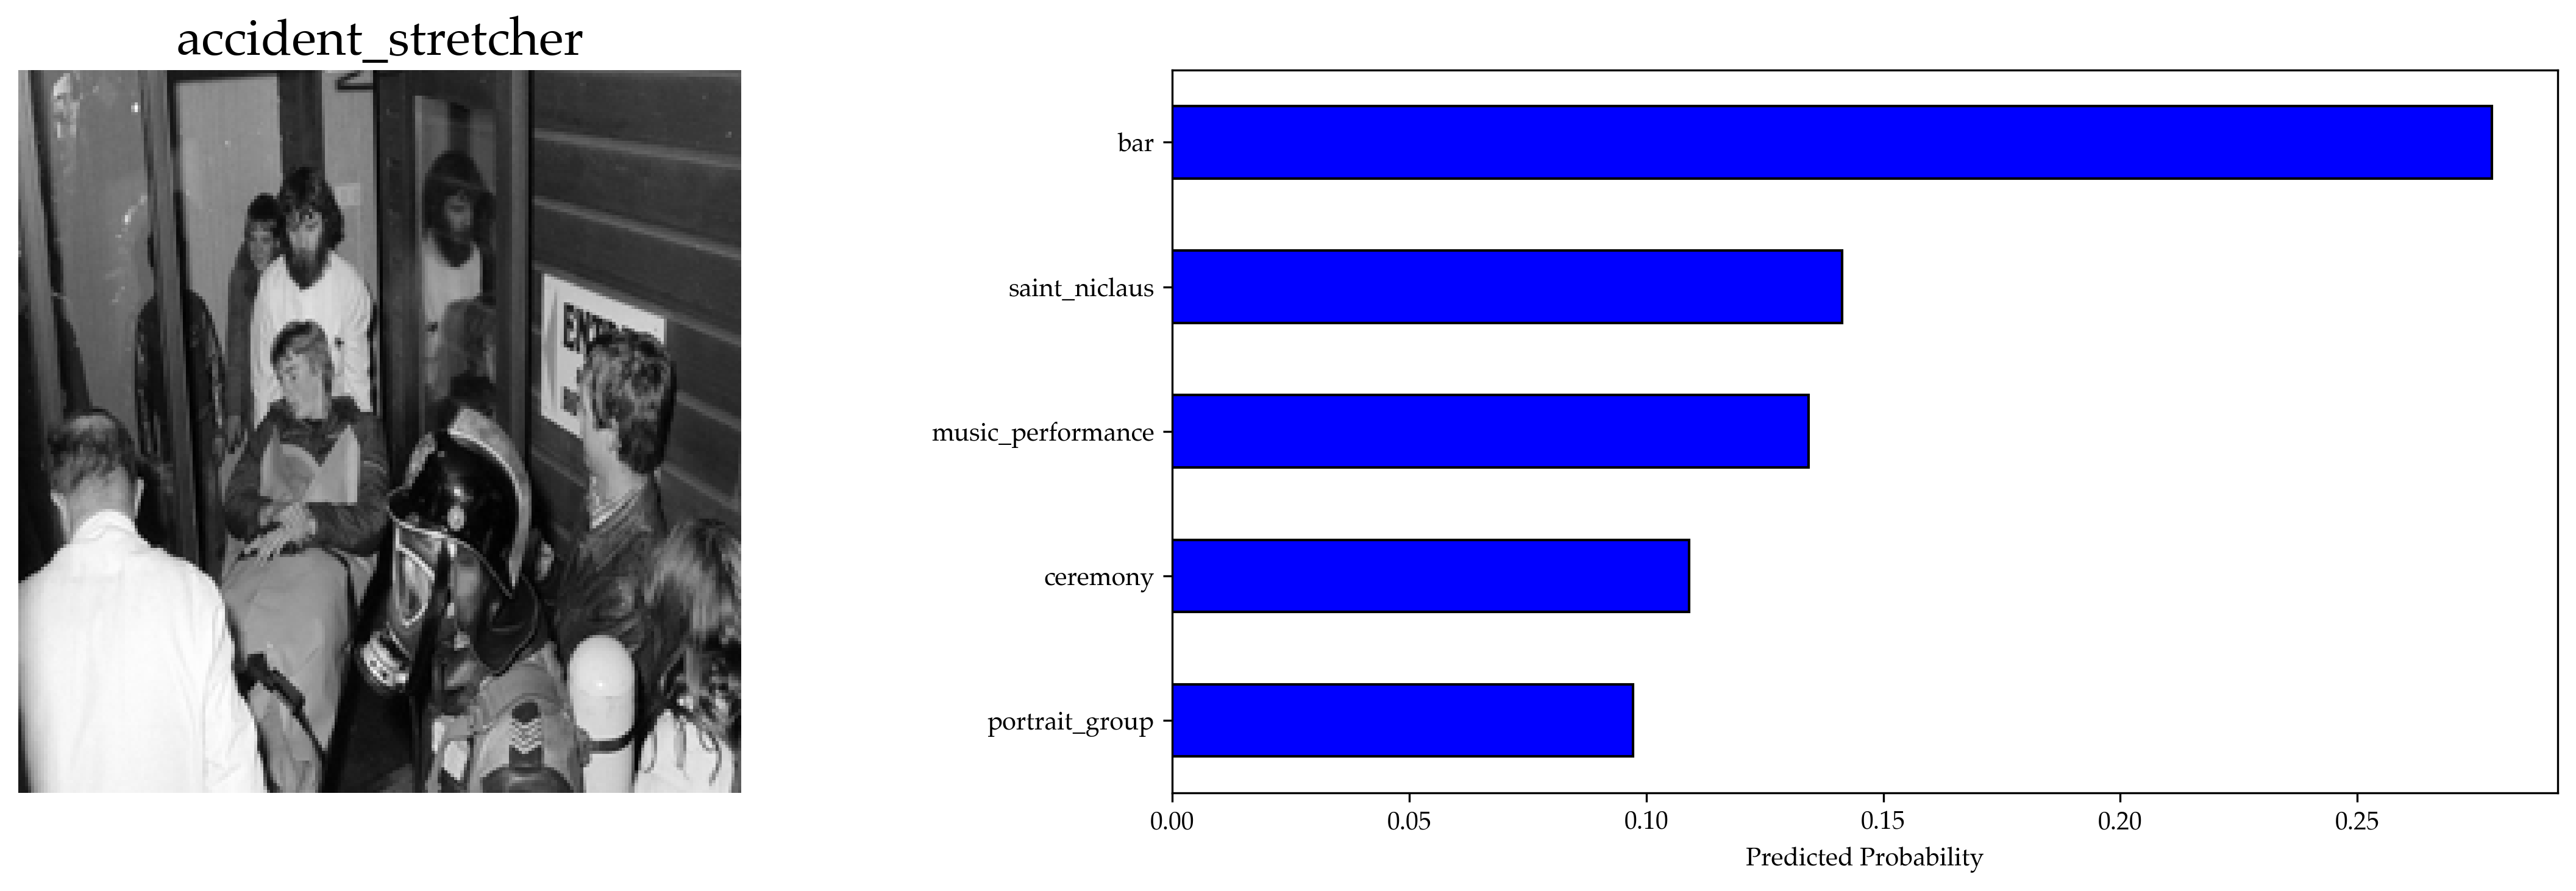
\includegraphics[width=0.9\textwidth]{../output/figures/accident_stretcher_example.png}
%  	\caption{Top5 predictions for a picture with the label `Accident stretcher.}
%  	\label{fig:top20}
%\end{figure}
%
%There were no categories with a top5-accuracy of 0. Figure~\ref{fig:top20} shows the top1-accuracy of the top 20 categories along with their number of training items. From this figure, we learn that these top categories not necessarily resulted from a large number of training data. Moreover, it seems that sports categories, e.g. basketball, cricket, soccer, etc., are detected with high accuracy. 
%
%\begin{figure}
%	\centering
%  	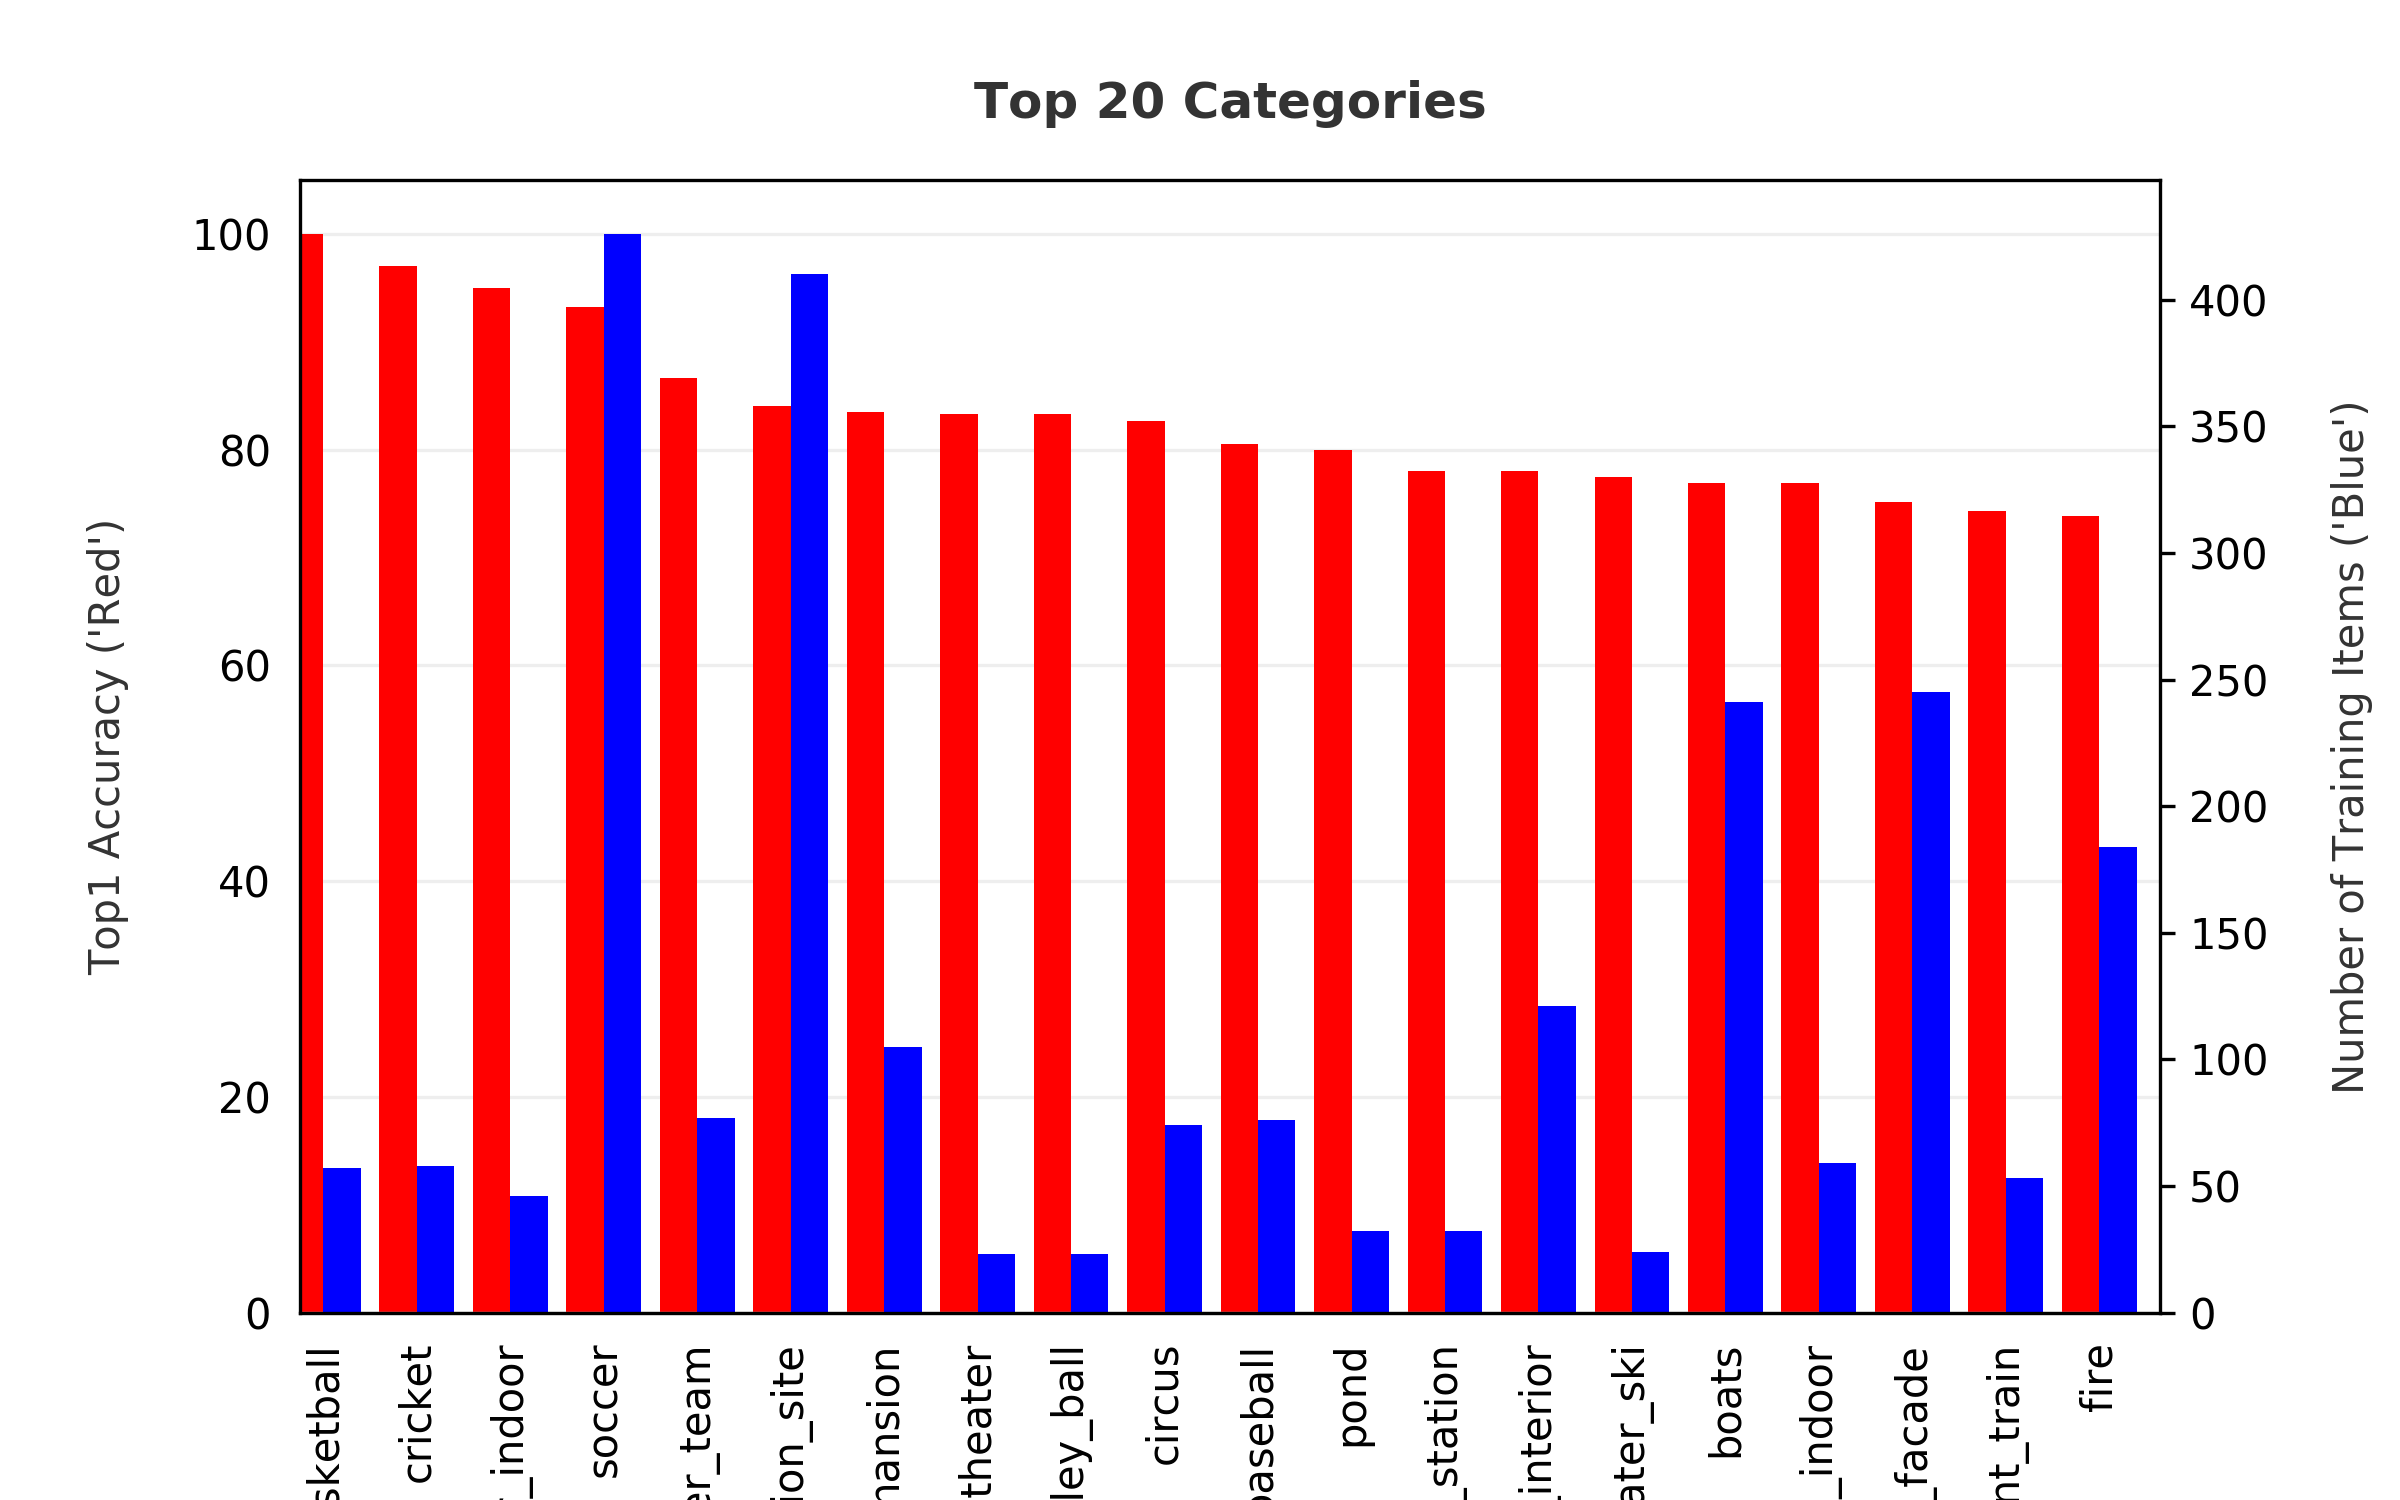
\includegraphics[width=0.9\textwidth]{../output/figures/top20.png}
%  	\caption{Top 20 categories and their top1-accuracy (red) and their training size (blue).}
%  	\label{fig:top20}
%\end{figure}
%
%Figure~\ref{fig:top5} shows the categories that score an top5-accuracy of .8 or higher. 
%
%\begin{figure}
%	\centering
%  	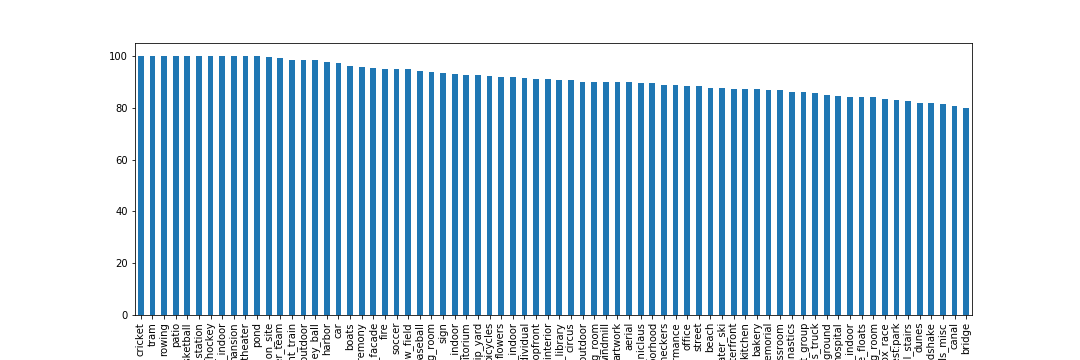
\includegraphics[width=0.80\textwidth]{../output/figures/top5_accuracy.png}
%  	\caption{Categories with top5-accuracy of >= .8}
%  	\label{fig:top5}
%\end{figure}
%
%There is also positive correlation between the number of training items and the accuracy, suggesting that with more training data, we can further improve the accuracy of the categories with fewer images. 
%
%
%
%\section{Discussion}
%
%During the second phase of the project we will digitize the entire photo collection and for a subset of these images, we will use groups of annotators to provide them with annotations.
%
%\section{Appendix}
%
%Here we list our annotation guides lines per categories. Some of these categories have been not been included in the training, because they included fewer than 10 images. 
%
%\subsubsection*{Accident Car}
%Traffic accident involving an automobile
%
%\subsubsection*{Accident Stretcher}
%Accident involving an person on a stretcher
%
%\subsubsection*{Accident Train}
%Traffic accident involving an train
%
%\subsubsection*{Aerial}
%Picture with an aerial perspective
%
%\subsubsection*{Airplane welcome}
%Pictures of people exiting a plane. These often included celebrities. 
%
%\subsubsection*{Amphitheater}
%The collection contains many pictures taken at an outside amphitheater in Bloemendaal. 
%
%\subsubsection*{Animals cow}
%Pictures cow live and dead cows.
%
%\subsubsection*{Animals dog}
%Pictures of dogs
%
%\subsubsection*{Animals horse}
%Pictures of horses
%
%\subsubsection*{Animals misc}
%Animals that do not fit in the previous categories. For final dataset, this might be subdivided in more categories.
%
%\subsubsection*{Artwork}
%Artwork without people, the focus is on the art work.
%There is also a separate category for statues. 
%
%
%\subsubsection*{Auditorium}
%Public building (used for speeches, performances) where audience sits. Pictures with and without audiences
%Overlap with categories `conference room` and `speech'
%
%\subsubsection*{Badminton}
%People playing badminton
%
%\subsubsection*{Bakery}
%Photos inside bakery, baking bread, presenting bread indoor/outdoors
%Overlap with Kitchen
%
%\subsubsection*{Bar}
%Area where drinks are served/consumed
%Overlap with Dining Room/Game Room
%
%\subsubsection*{Baseball}
%People playing baseball
%
%\subsubsection*{Baseball team}
%pictures of the baseball team, posing for a portrait.
%
%\subsubsection*{Basketball}
%People playing basketball. 
%
%\subsubsection*{Basketball team}
%pictures of the basketball team, posing for a portrait.
%
%\subsubsection*{Beach}
%If the beach is the picture's main focus, we select beach. Dunes is a separate category. Overlap with crowd/horse/running. When there is only water visible, we still select Beach. Possibly `sea' or `ocean' as a category.
%
%\subsubsection*{Bedroom}
%Images taken within bedrooms, i.e. must feature a bed
%
%\subsubsection*{Beauty Salon}
%Images that feature hairdressers or beauty salons
%
%\subsubsection*{Bicycles}
%Features bicycles or people riding bicycles
%Overlap with cycling, category for professional cycling and street/
%
%\subsubsection*{Boat Deck}
%Picture that focus on the deck of a boat, either with or without people. Not showing entire ship/boat from a distance. Overlap with boats category.
%
%\subsubsection*{Boats}
%Category focusing on a boat or multiple boats.
%Overlap with harbor/shipyard. If boat is harboured and harbor is taking up large area of picture. Shipyard depicts construction area for boats, boats under construction
%Overlap with beach, canal, river, waterfront. Difference is focus on boat
%
%\subsubsection*{Bookstore\/library}
%Bookstore or library as a combined category, as they are often difficult to separate. The pictures feature rows of books and/or people reading.
%Overlap with office, room which also often features books.
%
%\subsubsection*{Bowling}
%People bowling
%
%\subsubsection*{Boxing ring}
%Area for boxing matches.
%
%\subsubsection*{Bridge}
%Picture should feature a bridge as a central element
%Overlap with street/canal/river/boat
%
%\subsubsection*{Building Facade}
%Depicting the facade of a building/rows of buildings. Not showing the full building from a distance. Overlap with residential area/mansion. Latter are single large house, former pictures of areas without a clear focus on the facade. Overlap shopping area/residential area/mansion
%
%\subsubsection*{Bus Station}
%Area where busses depart. 
%
%\subsubsection*{Bus Stop}
%Area where busses stop. 
%
%\subsubsection*{Bus truck}
%Focus on large busses and trucks. Overlap with street
%
%\subsubsection*{Butchers shop}
%Butcher shop from inside, or people preparing meat. Overlap with animals/shopfront/shop/kitchen
%
%\subsubsection*{Campsite}
%People camping using tents/caravans etc.
%
%\subsubsection*{Canal}
%Flow of water, also includes natural flow of water rivers. Overlap with bridge/river/boat/fishing/waterfront
%
%\subsubsection*{Car}
%Pictures that focus on a car
%
%\subsubsection*{Car shop}
%Showroom in which cars are sold 
%
%\subsubsection*{Casino}
%People gambling in a casino, playing black jack, slots, or roulette.
%
%\subsubsection*{Castle}
%Pictures of a castle, or ruins of a castle.
%
%\subsubsection*{Catwalk}
%Models on a catwalk
%
%\subsubsection*{Cemetery}
%Pictures taken of a cemetery. Important element includes tombs, or tomb stones. 
%
%\subsubsection*{Ceremony}
%A group of people bundled together for a ceremony. This could be awards, flowers, or a medal. Note that there is also a specific category for hand shakes. 
%
%\subsubsection*{Chess checkers}
%People playing either chess or checkers. These are visually quite similar, for larger dataset, this category might be divided into two, if there are enough images.
%
%\subsubsection*{Church Indoor}
%Pictures taken inside a church. This could include masses, but also view of the church without people. 
%
%\subsubsection*{Church Outdoor}
%Pictures of the church/cathedral building.
%
%\subsubsection*{Circus}
%Pictures taken of a circus, inside of a circus tent. The outside of the circus tent is categorized as tent. 
%
%\subsubsection*{City Hall Stairs}
%Pictures taken of a group of people on the stairs outside of the city hall of Haarlem. This is quite a specific categories, but there are quite a few pictures that fit this category. 
%
%\subsubsection*{Classroom}
%Students inside a classroom
%
%\subsubsection*{Clergy}
%Pictures of clergy indoors or outdoors.
%
%\subsubsection*{Coffin}
%Pictures of deceased people in a coffin. 
%
%\subsubsection*{Construction site}
%Construction site, this also includes pictures of demolitions. It is quite difficult to separate the two visually. If enough images of both, we could separate the two. 
%
%\subsubsection*{Courtyard}
%Area between buildings, or outside yard in a group of buildings. 
%
%\subsubsection*{Circus}
%Pictures taken of a circus, inside of a circus tent. The outside of the circus tent is categorized as tent.  
%
%\subsubsection*{Cricket}
%People playing cricket
%
%\subsubsection*{Crosswalk}
%People crossing street, ‘zebra’ must be visible, otherwise street might be better
%
%\subsubsection*{Crowd}
%Gathering of people, where individuals are not clearly discernible. When posing for picture put in portrait category.
%
%\subsubsection*{Cycling}
%Professional cyclists
%
%\subsubsection*{Dancing}
% People dancing
% Overlap with bar, music performance, plaza
%
%\subsubsection*{Dining Room}
%Area where people eat, both in restaurants and houses
%
%\subsubsection*{Dorm room}
%Area with multiple beds, often bunk beds. 
%
%\subsubsection*{Drive Way}
%Drive way in front of buildings
%
%\subsubsection*{Dunes}
% Photos of dunes.
% Overlap with parade/memorial/crowd
%
%\subsubsection*{Excavation}
% People digging up something, archeological finds
% Overlap with construction site
%
%\subsubsection*{Exhibition}
%Room with artwork(s) and people. The focus is more clearly on the setting
%
%\subsubsection*{Factory indoor}
%Pictures taken with factories/assembly lines/production facilities
%
%\subsubsection*{Fair}
%Fun fairs
%
%\subsubsection*{Farm}
% Buildings surrounded by pasture/animals/crops
%
%\subsubsection*{Farm field}
% People working in farm fields/pictures of crops/farm fields
% Overlap with animals
%
%\subsubsection*{Field Hockey}
% People playing field hockey
%
%\subsubsection*{Field hockey team}
% Pictures of field hockey teams
%
%\subsubsection*{Fire}
%Pictures of fires, or building destroyed by fires. 
%
%\subsubsection*{Fishery}
% Pictures of fishing industry
%
%\subsubsection*{Fishing}
% People fishing
%
%\subsubsection*{Flag}
% People holding or raising flags
% Overlap with parade in which people hold flags
%
%\subsubsection*{Flowers}
% Pictures that include flowers
%
%\subsubsection*{Forest/Park}
%Picture taken in a forest or park
%
%\subsubsection*{Fountain}
% Pictures of fountains
%
%\subsubsection*{Funeral}
%Pictures of a funeral. Similar to memorial and cemetery. Here we only choose pictures that show a casket or burial itself.Overlap with memorial, parade, cemetery, flowers, church indoor
%
%\subsubsection*{Garbage Dump}
%
%\subsubsection*{Gas Station}
%
%\subsubsection*{Gymnastics}
%People performing gymnastics indoor and outdoor
%Overlap with circus/dancing
%
%\subsubsection*{Handshake}
%People shaking hands, subcategory of ceremony. 
%
%\subsubsection*{Harbor}
%Ships docked at a harbor, focus is not ships, but context of the harbor. 
%Overlap with boats and waterfront > waterfront is focus is on waterfront/kade
%
%\subsubsection*{Historical plays}
%People dressed up in historical garment enacting historical plays
%
%
%\subsubsection*{Hospital}
%Pictures taken in a hospital/dentist/medical lab setting
%
%\subsubsection*{House Boat}
%Pictures of the outside of house boats.
%
%\subsubsection*{Ice Skating}
%People skating on ice
%
%\subsubsection*{Kitchen}
% People in kitchen, preparing food
% Overlap with butcher\_store
%
%\subsubsection*{Korfbal}
% People playing korfbal, a dutch variant of basketball.
% 
% \subsubsection*{Laboratory}
%
%\subsubsection*{Lighthouse}
%
%\subsubsection*{Living room}
% People situated in a living room space.
% Overlap with portraits, which are often taken in a living room. To learn the living room category, I placed pictures in here taken in living rooms, with enough information on the living room. Overlap with portrait
%
%\subsubsection*{Mansion}
%Large houses, separated from housing blocks
%
%\subsubsection*{Market indoor}
% Indoor market/shopping fair
%
%\subsubsection*{Market outdoor}
% Outdoor market
% Overlap with crowd
%
%\subsubsection*{Marriage}
%Depicting a marriage couple, marriage ceremony
%Overlap with portrait group
%
%\subsubsection*{Martial Arts Gym}
%Space where people fight, judo/karate
%
%\subsubsection*{Meeting Room}
%Setting features meeting table with people sitting around it
%
%\subsubsection*{Memorial}
% Depicting a memorial site. Overlap with funeral/flowers/flag
%
%\subsubsection*{Military}
%Pictures depicting military personnel or military equipment. Overlap with parade and bus/trucks
%
%\subsubsection*{Motorcycle}
%Depicting motorcycle(s)
%
%\subsubsection*{Movie set}
%Depicting movie sets
%
%\subsubsection*{Musical Performance}
% People performing music
% Overlap with dance
%
%\subsubsection*{Office}
%Pictures set in an office environment
%
%\subsubsection*{Parade}
%People parading, marching bands
%
%\subsubsection*{Parade float}
%Pictures with flower trucks/floats
%
%\subsubsection*{Patio}
%People on patio’s sitting
%
%\subsubsection*{Playground}
% People/Children playing in a playground. Overlap with funfair and portrait children
% 
% \subsubsection*{Playing Cards}
%People playing cards
%
%\subsubsection*{Pond}
% Scenery of a pond. Overlap with canal/river/park
%
%\subsubsection*{Portrait Child}
% One child
%
%\subsubsection*{Portrait Children}
% One or more children
%
%\subsubsection*{Portrait Individual}
%
%\subsubsection*{Portrait Group}
%
%\subsubsection*{Protest}
%People protesting, banners clear signal
%
%\subsubsection*{Racecourse}
% Pictures taken on racecourse. Also category soapbox race
% Overlap with car, accident. 
%
%\subsubsection*{Railroad track}
%Pictures of the railroad track. There’s is also a category for trains.
%
%\subsubsection*{Repair Shop}
%Indoor pictures of repair shop, showing person repairing objects
%
%\subsubsection*{Residential neighborhood}
% Living area. Overlap with street/building facade
%
%\subsubsection*{Rowing}
% People rowing
%
%\subsubsection*{Running}
% People running in a sports event
%
%\subsubsection*{Saint Niclaus}
% Pictures of the Saint Niclaus festivities
%
%\subsubsection*{Shed}
%Wooden buildings, beach houses, living trailers
%
%\subsubsection*{Shipyard}
%Construction area for ships. Overlap with boats and harbor. 
%
%\subsubsection*{Shop interior}
%Photos of different kinds of shop interiors. 
%
%\subsubsection*{Shop front}
%Picture of a shop front, ‘etalage’
%
%\subsubsection*{Shopping street}
%Depicting street of shops/shoppers
%
%\subsubsection*{Sign}
%Signs, plaques, maps
%
%\subsubsection*{Snooker}
%People playing snooker, or billiards.
%
%\subsubsection*{Snowfield}
%Scenes set in snow, people skiing, sledding
%
%\subsubsection*{Soapbox Race}
%
%\subsubsection*{Soccer}
%people playing soccer
%
%\subsubsection*{Soccer Indoor}
%People playing indoor soccer
%
%\subsubsection*{Soccer Team}
%Portrait of soccer team
%
%\subsubsection*{Speech}
%Focus on person specking
%
%\subsubsection*{Statue}
%Pictures of sculptures/statues
%
%\subsubsection*{Street}
%Depicting street sceneries. Overlap with car, residential neighbourhood 
%
%\subsubsection*{Surfing}
%Depicting street sceneries. Overlap with car, residential neighbourhood 
%
%\subsubsection*{Swimming Pool Indoor}
%
%\subsubsection*{Swimming Pool Outdoor}
%
%\subsubsection*{Swimming Team}
%Portrait of a swimming team
%
%\subsubsection*{Table Tennis}
%
%\subsubsection*{Telecom}
%Pictures taken in radio studios, switchboards etc.
%
%\subsubsection*{Tent}
%Large tents, small tents should be placed in category campsite.
%
%\subsubsection*{Theatre}
%Plays performed in a theatre setting
%
%\subsubsection*{Tower}
%Pictures of towers, not church towers. 
%
%\subsubsection*{Train}
%Pictures of trains. Overlap with train station
%
%\subsubsection*{Train interior}
%Pictures of interiors of trains.
%
%\subsubsection*{Train station}
%Pictures of train stations, trains at stations etc..
%
%\subsubsection*{Tram}
%Pictures of trams
%
%\subsubsection*{Volley ball}
%Pictures of people playing volley ball
%
%\subsubsection*{Water Polo}
%People playing water polo
%
%\subsubsection*{Water ski}
%People on water skis
%
%\subsubsection*{Water Front}
%Scenes that focus on the water front
%
%\subsubsection*{Windmill}
%Pictures that contain a windmill

\end{document}
